\documentclass[10pt,border=4pt]{standalone}
\usepackage{mathptmx}
\usepackage{amsmath,amssymb,bm}
\usepackage{tikz}
\usetikzlibrary{patterns,decorations.pathmorphing,decorations.pathreplacing,arrows.meta,fit,backgrounds,calc,positioning,shapes.geometric}
\definecolor{acc}{HTML}{0B5394}
\definecolor{accl}{HTML}{EAF0F7}
\definecolor{grp}{HTML}{F5F5F5}
\definecolor{org}{HTML}{C55A11}
\definecolor{orgl}{HTML}{FBEFE6}
\tikzset{
 dat/.style={draw=black,line width=0.6pt,fill=white,align=center,font=\small,inner sep=3pt,minimum height=0.85cm},
 lay/.style={draw=acc,line width=0.8pt,fill=accl,rounded corners=2pt,align=center,font=\small,inner sep=3pt,minimum height=0.85cm},
 cnd/.style={draw=org,line width=0.8pt,fill=orgl,rounded corners=2pt,align=center,font=\small,inner sep=3pt,minimum height=0.75cm},
 op/.style={circle,draw=black,line width=0.6pt,fill=white,inner sep=0.5pt,font=\small,minimum size=5mm},
 grpb/.style={draw=black!45,dashed,line width=0.6pt,rounded corners=3pt,inner sep=6pt},
 arr/.style={-{Latex[length=2.2mm,width=1.7mm]},line width=0.7pt},
 carr/.style={-{Latex[length=2.2mm,width=1.7mm]},line width=0.7pt,draw=org},
 shp/.style={font=\scriptsize,text=black!70,inner sep=1pt},
 lab/.style={font=\footnotesize,inner sep=1pt},
 ttl/.style={font=\small\bfseries,inner sep=0pt,anchor=west}
}
\newcommand{\xh}{\mathbf{x}_h}\newcommand{\xf}{\mathbf{x}_f}

\tikzset{vlv/.style={draw=org,line width=0.8pt,fill=orgl,minimum width=1.25cm,minimum height=0.6cm,font=\footnotesize,inner sep=1pt},
 vlh/.style={draw=black!60,line width=0.8pt,fill=grp,minimum width=1.25cm,minimum height=0.6cm,font=\footnotesize,inner sep=1pt},
 cyl/.style={draw=acc,line width=0.8pt,fill=accl,align=center,font=\small,minimum height=1.2cm,minimum width=2.0cm},
 flow/.style={-{Latex[length=2.2mm,width=1.7mm]},line width=1pt,draw=acc}}
\begin{document}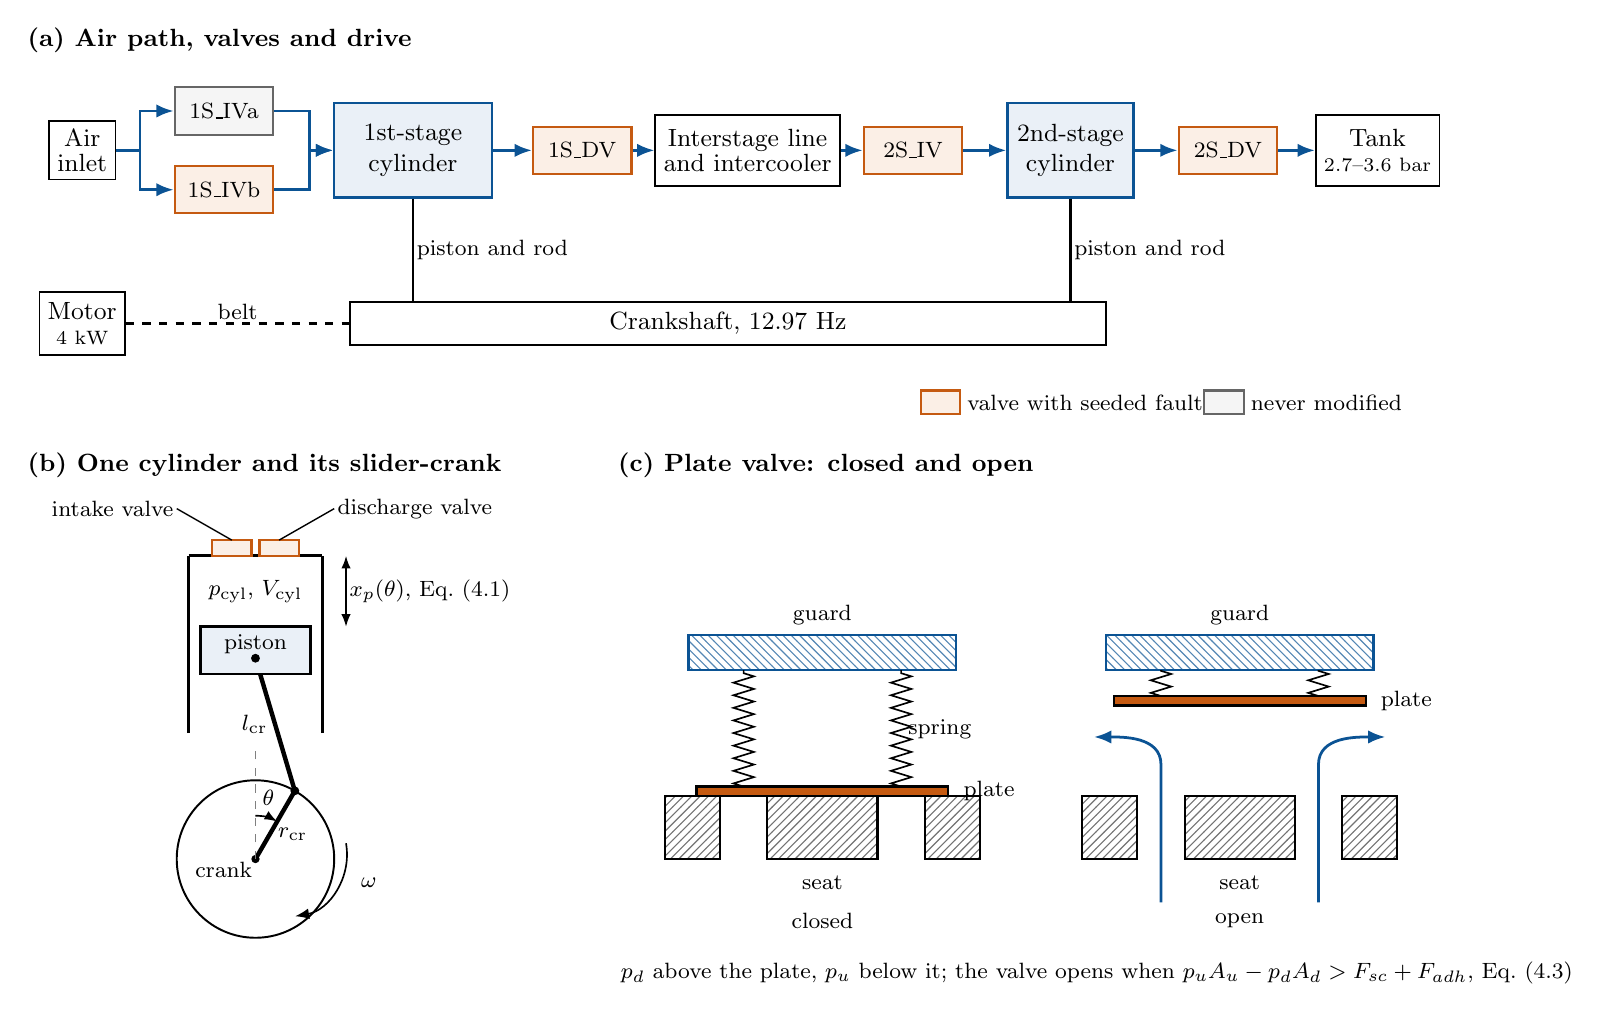
\begin{tikzpicture}[x=1cm,y=1cm]
% ---------------- (a) air path
\node[ttl] at (-0.3,3.0) {(a) Air path, valves and drive};
\node[dat,minimum height=0.7cm] (in) at (0.4,1.6) {Air\\[-2pt]inlet};
\node[vlh] (iva) at (2.2,2.1) {1S\_IVa};
\node[vlv] (ivb) at (2.2,1.1) {1S\_IVb};
\node[cyl] (c1) at (4.6,1.6) {1st-stage\\cylinder};
\node[vlv] (dv1) at (6.75,1.6) {1S\_DV};
\node[dat,minimum height=0.9cm] (ic) at (8.85,1.6) {Interstage line\\[-2pt]and intercooler};
\node[vlv] (iv2) at (10.95,1.6) {2S\_IV};
\node[cyl,minimum width=1.6cm] (c2) at (12.95,1.6) {2nd-stage\\cylinder};
\node[vlv] (dv2) at (14.95,1.6) {2S\_DV};
\node[dat,minimum height=0.9cm] (tk) at (16.85,1.6) {Tank\\[-2pt]\scriptsize 2.7--3.6 bar};
\draw[flow] (in.east)--++(0.3,0)|-(iva.west); \draw[flow] (in.east)--++(0.3,0)|-(ivb.west);
\draw[flow] (iva.east)-|([xshift=-3mm]c1.west)--(c1.west); \draw[flow] (ivb.east)-|([xshift=-3mm]c1.west)--(c1.west);
\draw[flow] (c1)--(dv1); \draw[flow] (dv1)--(ic); \draw[flow] (ic)--(iv2); \draw[flow] (iv2)--(c2); \draw[flow] (c2)--(dv2); \draw[flow] (dv2)--(tk);
% drive
\node[dat,minimum height=0.8cm] (mot) at (0.4,-0.6) {Motor\\[-2pt]\scriptsize 4 kW};
\node[dat,minimum width=9.6cm,minimum height=0.55cm] (cs) at (8.6,-0.6) {Crankshaft, 12.97 Hz};
\draw[line width=0.9pt,dashed] (mot.east)--node[lab,above]{belt}(cs.west);
\draw[line width=0.8pt] (c1.south)--node[lab,right]{piston and rod}(c1.south|-cs.north);
\draw[line width=0.8pt] (c2.south)--node[lab,right]{piston and rod}(c2.south|-cs.north);
% legend
\node[vlv,minimum width=0.5cm,minimum height=0.3cm] (l1) at (11.3,-1.6) {}; \node[lab,anchor=west] at (11.6,-1.6) {valve with seeded faults};
\node[vlh,minimum width=0.5cm,minimum height=0.3cm] (l2) at (14.9,-1.6) {}; \node[lab,anchor=west] at (15.2,-1.6) {never modified};
% ---------------- (b) slider-crank
\begin{scope}[shift={(0,-7.4)}]
\node[ttl] at (-0.3,5.0) {(b) One cylinder and its slider-crank};
\coordinate (O) at (2.6,0);
\draw[line width=0.7pt] (O) circle (1.0); \fill (O) circle (1.5pt) node[lab,below left]{crank};
\coordinate (C) at ($(O)+(60:1.0)$);
\draw[line width=1.6pt] (O)--node[lab,below right=-1pt]{$r_\text{cr}$}(C);
\coordinate (Pp) at (2.6,2.55);
\draw[line width=1.6pt] (C)--node[lab,left=1pt]{$l_\text{cr}$}(Pp); \fill (C) circle (1.6pt); 
\draw[line width=0.9pt,fill=accl] (1.9,2.35) rectangle (3.3,2.95); \fill (Pp) circle (1.6pt); \node[lab] at (2.6,2.73) {piston};
\draw[line width=1pt] (1.75,1.6)--(1.75,3.85) (3.45,1.6)--(3.45,3.85);
\draw[line width=1pt] (1.75,3.85)--(2.05,3.85) (2.55,3.85)--(2.65,3.85) (3.15,3.85)--(3.45,3.85);
\draw[line width=0.8pt,draw=org,fill=orgl] (2.05,3.85) rectangle (2.55,4.05); \draw[line width=0.8pt,draw=org,fill=orgl] (2.65,3.85) rectangle (3.15,4.05);
\draw[line width=0.5pt] (2.3,4.05)--(1.6,4.45) node[lab,anchor=east]{intake valve}; \draw[line width=0.5pt] (2.9,4.05)--(3.6,4.45) node[lab,anchor=west]{discharge valve};
\draw[dashed,black!50] (O)--++(0,1.4); \draw[-{Latex[length=1.6mm]},line width=0.6pt] ($(O)+(0,0.55)$) arc (90:60:0.55); \node[lab] at ($(O)+(78:0.8)$) {$\theta$};
\draw[{Latex[length=1.6mm]}-{Latex[length=1.6mm]},line width=0.6pt] (3.75,3.85)--node[lab,right]{$x_p(\theta)$, Eq.~(4.1)}(3.75,2.95);
\node[lab] at (2.6,3.4) {$p_\text{cyl}$, $V_\text{cyl}$};
\draw[-{Latex[length=1.8mm]},line width=0.6pt] (3.75,0.2) arc (10:-80:0.8); \node[lab,anchor=west] at (3.9,-0.3) {$\omega$};
\end{scope}
% ---------------- (c) plate valve
\begin{scope}[shift={(7.8,-7.4)}]
\node[ttl] at (-0.6,5.0) {(c) Plate valve: closed and open};
\foreach \dx/\op/\tt in {0/0/closed, 5.3/1/open}{
 \begin{scope}[shift={(\dx,0)}]
 % seat with two ports
 \fill[pattern=north east lines,pattern color=black!55] (0,0) rectangle (0.7,0.8) (1.3,0) rectangle (2.7,0.8) (3.3,0) rectangle (4.0,0.8);
 \draw[line width=0.8pt] (0,0) rectangle (0.7,0.8) (1.3,0) rectangle (2.7,0.8) (3.3,0) rectangle (4.0,0.8);
 \node[lab] at (2.0,-0.3) {seat};
 % guard
 \fill[pattern=north west lines,pattern color=acc!70] (0.3,2.4) rectangle (3.7,2.85);
 \draw[line width=0.8pt,draw=acc] (0.3,2.4) rectangle (3.7,2.85); \node[lab] at (2.0,3.1) {guard};
 % plate
 \pgfmathsetmacro{\py}{0.8+\op*1.15}
 \draw[line width=0.8pt,fill=org] (0.4,\py) rectangle (3.6,\py+0.12);
 % springs
 \foreach \sx in {1.0,3.0}{\draw[line width=0.6pt,decorate,decoration={zigzag,segment length=1.6mm,amplitude=1.3mm}] (\sx,\py+0.12)--(\sx,2.4);}
 \node[lab,anchor=west] at (3.75,\py+0.06) {plate}; \ifnum\op=0 \node[lab,anchor=west] at (3.05,{(\py+2.5)/2}) {spring};\fi
 \node[lab,anchor=north] at (2.0,-0.65) {\tt};
 \ifnum\op=1
   \draw[flow,draw=acc] (1.0,-0.55)--(1.0,1.2) to[out=90,in=0] (0.15,1.55); \draw[flow,draw=acc] (3.0,-0.55)--(3.0,1.2) to[out=90,in=180] (3.85,1.55);
 \fi
 \end{scope}}
\node[lab,align=left,anchor=west] at (-0.6,-1.45) {$p_d$ above the plate, $p_u$ below it; the valve opens when $p_uA_u-p_dA_d>F_{sc}+F_{adh}$, Eq.~(4.3)};
\end{scope}
\end{tikzpicture}\end{document}
